% v2-acmsmall-sample.tex, dated March 6 2012
% This is a sample file for ACM small trim journals
%
% Compilation using 'acmsmall.cls' - version 1.3 (March 2012), Aptara Inc.
% (c) 2010 Association for Computing Machinery (ACM)
%
% Questions/Suggestions/Feedback should be addressed to => "acmtexsupport@aptaracorp.com".
% Users can also go through the FAQs available on the journal's submission webpage.
%
% Steps to compile: latex, bibtex, latex latex
%
% For tracking purposes => this is v1.3 - March 2012

\documentclass[prodmode,acmtecs]{acmsmall} % Aptara syntax

\usepackage{graphicx}
\usepackage{caption}
\usepackage{subfigure}
\usepackage{setspace}
\usepackage{tabulary}
\usepackage{fancybox}
\usepackage{enumitem}

% font in listings
\usepackage{courier}

\makeatletter
\newenvironment{CenteredBox}{% 
\begin{Sbox}}{% Save the content in a box
\end{Sbox}\centerline{\parbox{\wd\@Sbox}{\TheSbox}}}% And output it centered
\makeatother

\let\proof\relax
\let\endproof\relax
\usepackage{amsthm}
\newcommand{\specialcell}[2][c]{%
  \begin{tabular}[#1]{@{}c@{}}#2\end{tabular}}

\usepackage{lineno}
\usepackage{xfrac}

% Theorems, definitions, lemmas, etc
\newtheorem{Def}{Definition}
\newtheorem{Prop}{Proposition}
\newtheorem{Algo}{Algorithm}
\newtheorem{Const}{Constraint}
\newtheorem*{Rem*}{Remark}

\usepackage{alltt}
\renewcommand{\ttdefault}{txtt}

% line over text in non math mode
\newcommand{\textoverline}[1]{$\overline{\mbox{#1}}$}

\usepackage{listings}
\lstset{language=C, breaklines=true, mathescape,
			 morekeywords={each,min,not}}

\usepackage[cmex10]{amsmath}
\usepackage{url}

% Metadata Information
%\acmVolume{9}
%\acmNumber{4}
%\acmArticle{39}
%\acmYear{2010}
%\acmMonth{3}

% Document starts
\begin{document}

% Page heads
\markboth{F. Luporini et al.}{On Optimality of Finite Element Integration}

% Title portion
\title{On Optimality of Finite Element Integration}
\author{Fabio Luporini
\affil{Imperial College London}
David A. Ham
\affil{Imperial College London}
Paul H. J. Kelly
\affil{Imperial College London}}

\begin{abstract}
We tackle the problem of automatically generating optimal finite element integration routines given a high level specification of arbitrary multilinear forms. Optimality and quasi-optimality are defined in terms of floating point operations given a memory bound. We provide an approach to explore the space of legal transformations and discuss under what conditions optimality or quasi-optimality hold. A theoretical analysis and extensive experimentation, which shows systematic performance improvements over several state-of-the-art code generation systems, validate the approach.
\end{abstract}

\category{G.1.8}{Numerical Analysis}{Partial Differential Equations -
  Finite element methods}

\category{G.4}{Mathematical Software}{Parallel and vector implementations}

\terms{Design, Performance}

\keywords{Finite element integration, local assembly, compilers, performance optimization}

\acmformat{Fabio Luporini, David A. Ham, and Paul H. J. Kelly, 2015. On Optimality of Finite Element Integration.}

% At a minimum you need to supply the author names, year and a title.
% IMPORTANT: Full first names whenever they are known, surname last,
% followed by a period.  In the case of two authors, 'and' is placed
% between them.  In the case of three or more authors, the serial
% comma is used, that is, all author names except the last one but
% including the penultimate author's name are followed by a comma, and
% then 'and' is placed before the final author's name.  If only first
% and middle initials are known, then each initial is followed by a
% period and they are separated by a space.  The remaining information
% (journal title, volume, article number, date, etc.) is
% 'auto-generated'.

\begin{bottomstuff}

This research is partly funded by the MAPDES project, by the
Department of Computing at Imperial College London, by EPSRC through
grants EP/I00677X/1, EP/I006761/1, and EP/L000407/1, by NERC grants
NE/K008951/1 and NE/K006789/1, by the U.S.  National Science
Foundation through grants 0811457 and 0926687, by the U.S. Army
through contract W911NF-10-1-000, and by a HiPEAC collaboration
grant. The authors would like to thank Mr. Andrew T.T. McRae,
Dr. Lawrence Mitchell, and Dr. Francis Russell for their invaluable
suggestions and their contribution to the Firedrake project.

Author's addresses: Fabio Luporini $\&$ Paul H. J. Kelly, Department of Computing,
Imperial College London; David A. Ham, Department of Computing and
Department of Mathematics, Imperial College London; 
\end{bottomstuff}

\maketitle


\section{Introduction}

The need for rapid implementation of high performance, robust, and portable finite element methods has led to approaches based on automated code generation. This has been proven successful in the context of the FEniCS (\cite{Fenics}) and Firedrake (\cite{firedrake-paper}) projects. In these frameworks, the weak variational form of a problem is expressed at high level by means of a domain-specific language. The mathematical specification is manipulated by a form compiler that generates a representation of assembly operators. By applying these operators to an element in the discretized domain, a local matrix and a local vector, which represent the contributions of that element to the equation approximated solution, are computed. The code for assembly operators must be carefully optimized: as the complexity of a variational form increases, in terms of number of derivatives, pre-multiplying functions, or polynomial order of the chosen function spaces, the operation count increases, with the result that assembly often accounts for a significant fraction of the overall runtime. 

As demonstrated by the substantial body of research on the topic, automating the generation of such high performance implementations poses several challenges. This is a result of the complexity inherent in the mathematical expressions involved in the numerical integration, which varies from problem to problem, and the particular structure of the loop nests enclosing the integrals. General-purpose compilers, such as \emph{GNU's} and \emph{Intel's}, fail at exploiting the structure inherent in the expressions, thus producing sub-optimal code (i.e., code which performs more floating-point operations, or ``flops'', than necessary; we show this is Section~\ref{sec:perf-results}). Research compilers, for instance those based on polyhedral analysis of loop nests such as PLUTO (\cite{PLUTO}), focus on parallelization and optimization for cache locality, treating issues orthogonal to the question of minimising flops. The lack of suitable third-party tools has led to the development of a number of domain-specific code transformation (or synthesizer) systems. In~\citeN{quadrature1}, it is shown how automated code generation can be leveraged to introduce optimizations that a user should not be expected to write ``by hand''. In~\citeN{FFC-TC} and~\citeN{Francis}, mathematical reformulations of finite element integration are studied with the aim of minimizing the operation count. In~\citeN{Luporini}, the effects and the interplay of generalized code motion and a set of low level optimizations are analysed. It is also worth mentioning an on-going effort to produce a new form compiler, called UFLACS (\cite{Uflacs}), which adds to the already abundant set of code transformation systems for assembly operators. The performance evaluation in Section~\ref{sec:perf-results} includes most of these optimization systems.

However, in spite of such a considerable research effort, still there is no answer to one fundamental question: can we automatically generate an implementation of a form which is optimal in the number of flops executed? In this paper, we formulate an approach that solves this problem for a particular class of forms and provides very good approximations (``quasi-optimality'') in all other cases. Summarizing, our contributions are as follows:

\begin{itemize}
\item We formalize finite element integration loop nests and we build the space of legal transformations impacting their operation count.
\item We provide an algorithm to select points in the transformation space. The algorithm uses a cost model to: (i) understand whether a transformation reduces or increases the operation count; (ii) choose between different (non-composable) transformations.
\item We explain under what conditions our algorithm leads to optimality. In particular, we show that (i) for a particular class of problems, optimality is reached; (ii) quasi-optimality is, in general, always achieved (i.e., the operation count is at least optimal in innermost loops).
\item We integrate our approach with a compiler, COFFEE\footnote{COFFEE stands for COmpiler For Fast Expression Evaluation. The compiler is open-source and available at \url{https://github.com/coneoproject/COFFEE}}, which is in use in the Firedrake framework.
\item We experimentally evaluate using a broader suite of forms, discretizations, and code generation systems than has been used in prior research. This is essential to demonstrate that our optimality model holds in practice.
\end{itemize}

In addition, in order to place COFFEE on the same level as other code generation systems from the viewpoint of low level optimization (which is essential for a fair performance comparison)

\begin{itemize}
\item We introduce an engine based on symbolic execution that allows skipping irrelevant floating point operations (e.g., those involving zero-valued quantities).
\end{itemize}


\section{Preliminaries}
\label{sec:background}
We review finite element integration using the same notation and examples adopted in~\citeN{quadrature1} and~\citeN{Francis}. 

We consider the weak formulation of a linear variational problem
\begin{equation}
\begin{split}
\text{Find}\ u \in U\ \text{such that} \\
a(u, v) = L(v), \forall v \in V
\end{split}
\end{equation}
where $a$ and $L$ are, respectively, a bilinear and a linear form. The set of \textit{trial} functions $U$ and the set of \textit{test} functions $V$ are discrete function spaces. For simplicity, we assume $U = V$. Let $\lbrace \phi_i \rbrace$ be the set of basis functions spanning $U$. The unknown solution $u$ can be approximated as a linear combination of the basis functions $\lbrace \phi_i \rbrace$. From the solution of the following linear system it is possible to determine a set of coefficients to express $u$:
\begin{equation}
Au = b
\end{equation}
in which $A$ and $b$ discretize $a$ and $L$ respectively:
\begin{equation}
\centering
\begin{split}
A_{ij} = a(\phi_i(x), \phi_j(x)) \\
b_i = L(\phi_i(x))
\end{split}
\end{equation}
The matrix $A$ and the vector $b$ are ``assembled'' and subsequently used to solve the linear system through (typically) an iterative method.

We focus on the assembly phase, which is often characterized as a two-step procedure: \textit{local} and \textit{global} assembly. Local assembly is the subject of this article. It consists of computing the contributions of a single element in the discretized domain to the equation approximated solution. In global assembly, such local contributions are ``coupled'' by suitably inserting them into $A$ and $b$. 

We illustrate local assembly in a concrete example, the evaluation of the local element matrix for a Laplacian operator. Consider the weighted Laplace equation
\begin{equation}
- \nabla \cdot (w \nabla u) = 0
\end{equation}
in which $u$ is unknown, while $w$ is prescribed. The bilinear form associated with the weak variational form of the equation is:
\begin{equation}
a(v, u) = \int_\Omega w \nabla v \cdot \nabla u\ \mathrm{d}x
\end{equation}
The domain $\Omega$ of the equation is partitioned into a set of cells (elements) $T$ such that $\bigcup T = \Omega$ and $\bigcap T = \emptyset$. By defining $\lbrace \phi_i^K \rbrace$ as the set of local basis functions spanning $U$ on the element $K$, we can express the local element matrix as
\begin{equation}
\label{stiffness}
A_{ij}^K = \int_K w \nabla \phi_i^K \cdot \nabla \phi_j^K\ \mathrm{d}x
\end{equation}
The local element vector $L$ can be determined in an analogous way. 

\subsection{Monomials}
\label{sec:monomials}
In general, it has been shown (e.g., in~\citeN{Kirby:TC}) that local element tensors can be expressed as a sum of integrals over $K$, each integral being the product of derivatives of functions from sets of discrete spaces and, possibly, functions of some spatially varying coefficients. An integral of this form is called \textit{monomial}. 

%From the computational perspective, its evaluation is however less expensive than that of $A$.

\subsection{Quadrature mode}
Quadrature schemes are typically used to numerically evaluate $A_{ij}^K$. For convenience, a reference element $K_0$ and an affine mapping $F_K : K_0 \rightarrow K$ to any element $K \in T$ are introduced. This implies that a change of variables from reference coordinates $X_0$ to real coordinates $x = F_K (X_0)$ is necessary any time a new element is evaluated. The numerical integration routine based on quadrature over an element $K$ can be expressed as follows
\begin{equation}
\label{eq:quadrature}
A_{ij}^K = \sum_{q=1}^N \sum_{\alpha_3=1}^n \phi_{\alpha_3}(X^q)w_{\alpha_3} \sum_{\alpha_1=1}^d \sum_{\alpha_2=1}^d \sum_{\beta=1}^d \frac{\partial X_{\alpha_1}}{\partial x_{\beta}} \frac{\partial \phi_i^K(X^q)}{\partial X_{\alpha_1}} \frac{\partial X_{\alpha_2}}{\partial x_{\beta}} \frac{\partial \phi_j^K(X^q)}{\partial X_{\alpha_2}} det F_K' W^q
\end{equation}
where $N$ is the number of integration points, $W^q$ the quadrature weight at the integration point $X^q$, $d$ is the dimension of $\Omega$, $n$ the number of degrees of freedom associated to the local basis functions, and $det$ the determinant of the Jacobian matrix used for the aforementioned change of coordinates.  

% Magari la summation sui coefficients la sputo dentro? che dici?

\subsection{Tensor contraction mode}
\label{sec:tc}
Starting from Equation~\ref{eq:quadrature}, exploiting linearity, associativity and distributivity of the involved mathematical operators, we can rewrite the expression as
\begin{equation}
\label{eq:tensor}
A_{ij}^K = \sum_{\alpha_1=1}^d \sum_{\alpha_2=1}^d \sum_{\alpha_3=1}^n det F_K' w_{\alpha_3} \sum_{\beta=1}^d \frac{X_{\alpha_1}}{\partial x_{\beta}} \frac{\partial X_{\alpha_2}}{\partial x_{\beta}} \int_{K_0} \phi_{\alpha_3} \frac{\partial \phi_{i_1}}{\partial X_{\alpha_1}} \frac{\partial \phi_{i_2}}{\partial X_{\alpha_2}} dX.
\end{equation}
A generalization of this transformation has been proposed in~\cite{Kirby:TC}. Because of only involving reference element terms, the integral in the equation can be pre-evaluated and stored in temporary variables. The evaluation of the local tensor can then be abstracted as
\begin{equation}
A_{ij}^K = \sum_{\alpha} A_{i_1 i_2 \alpha}^0 G_{K}^\alpha
\end{equation}
in which the pre-evaluated ``reference tensor'' $A_{i_1 i_2 \alpha}$ and the cell-dependent ``geometry tensor'' $G_{K}^\alpha$ are exposed. 

\subsection{Qualitative comparison}
\label{sec:qualitative}
Depending on form and discretization, the relative performance of the two modes, in terms of the operation count, can vary quite dramatically. The presence of derivatives or coefficient functions in the input form tends to increase the size of the geometry tensor, making the traditional quadrature mode preferable for ``complex'' forms. On the other hand, speed-ups from adopting tensor mode can be significant in a wide class of forms in which the geometry tensor remains ``sufficiently small''. The discretization, particularly the relative polynomial order of trial, test, and coefficient functions, also plays a key role in the resulting operation count. 

These two modes have been implemented in the FEniCS Form Compiler (\cite{FFC-TC}). In this compiler, a heuristic is used to choose the most suitable mode for a given form. It consists of analysing each monomial in the form, counting the number of derivatives and coefficient functions, and checking if this number is greater than a constant found empirically (\cite{Fenics}). We will later comment on the efficacy of this approach (Section~\ref{sec:perf-results}). For the moment, we just recall that one of the goals of this research is to produce a system that goes beyond the dichotomy between quadrature and tensor modes. We will reason in terms of loop nests, code motion, and code pre-evaluation, searching the entire implementation space for an optimal synthesis.  

\section{Transformation Space}
\label{sec:optimal-impl}
In this section, we characterize optimality and quasi-optimality for finite element integration as well as the space of legal transformations that we need to explore to achieve it. How the exploration is performed is discussed in Section~\ref{sec:optimal-synthesis}. 

\subsection{Loop nests, expressions and optimality}
\label{sec:lnopt}
In order to make the article self-contained, we start with reviewing basic compiler terminology.

\begin{Def}[Perfect and imperfect loop nests]
A perfect loop nest is a loop whose body either 1) comprises only a sequence
of non-loop statements or 2) is itself a perfect loop nest. If this
condition does not hold, a loop nest is said to be imperfect. 
\end{Def}

\begin{Def}[Independent basic block]
An independent basic block is a sequence of statements such that no data
dependencies exist between statements in the block.
\end{Def}

We focus on perfect nests whose innermost loop body is an independent basic
block. A straightforward property of this class is that hoisting invariant
expressions from the innermost to any of the outer loops or the preheader
(i.e., the block that precedes the entry point of the nest) is always safe,
as long as any dependencies on loop indices are honored. We will make use of this property. The results of this section could also be generalized to larger classes of loop nests, in which basic block independence does not hold, although this would require refinements beyond the scope of this paper. 

By mapping mathematical properties to the loop nest level, we introduce the
concepts of a \textit{linear loop} and, more generally, a (perfect) multilinear loop nest.

\begin{Def}[Linear loop]
A loop $L$ defining the iteration space $I$ through the iteration variable $i$, or simply $L_i$, is linear if in its body
\begin{enumerate}
\item $i$ appears only as an array index, and
\item whenever an array $a$ is indexed by $i$ ($a[i]$), all expressions in which this appears are affine in $a$.
\end{enumerate}
\end{Def}

\begin{Def}[Multilinear loop nest]
A multilinear loop nest of arity $n$ is a perfect nest composed of $n$ loops, in which all of the expressions appearing in the body of the innermost loop are linear in each loop $L_i$ separately.
\end{Def}

We will show that multilinear loop nests, which arise naturally when translating bilinear or linear forms into code, are important because they have a structure that we can take advantage of to synthesize optimal code.

We define two other classes of loops. 

\begin{Def}[Reduction loop]
\label{def:i-loop}
A loop $L_i$ is said to be a reduction loop if in its body
\begin{enumerate}
\item $i$ appears only as an array index, and
\item for each augmented assignment statement $S$ (e.g., an increment), arrays indexed by $i$ appear only on the right hand side of $S$.
\end{enumerate}
\end{Def}

\begin{Def}[Free order loop]
\label{def:e-loop}
A loop $L_i$ is said to be a free order loop if its iterations can be executed in any arbitrary order; that is, there are no loop-carried dependencies across different iterations. 
\end{Def}

\begin{figure}\begin{CenteredBox}
\lstinputlisting[basicstyle=\footnotesize\ttfamily]{listings/loopnest.code}
\end{CenteredBox}\caption{The loop nest implementing a generic bilinear form.}\label{code:loopnest}\end{figure}

To contextualize, consider Equation~\ref{eq:quadrature} and the (abstract) loop nest implementing it illustrated in Figure~\ref{code:loopnest}. The imperfect nest $\Lambda=[L_e, L_i, L_j, L_k]$ comprises a free order loop $L_e$ (over elements in the mesh), a reduction loop $L_i$ (performing numerical integration), and a multilinear loop nest $[L_j, L_k]$ (over test and trial functions). In the body of $L_k$, one or more statements evaluate the local tensor for the element $e$. Expressions (right hand side of a statement) result from the translation of a form in high level matrix notation into code. In particular, $m$ is the number of ``terms'' (a monomial can be implemented by one or more terms), $\alpha_{eij}$ ($\beta_{eik}$) represents the product of a coefficient function (e.g., the inverse Jacobian matrix for the change of coordinates) with test (trial) functions, and $\sigma_{ei}$ is a function of coefficients and geometry. We do not pose particular restrictions on function spaces (e.g., scalar- or vector-valued), coefficients (e.g., linear or non-linear), differential and vector operators, so $\sigma_{ei}$ can be arbitrarily complex. We say that such an expression is in \textit{normal form}, because the algebraic structure of a variational form is intact (e.g., products have not been expanded yet, distinct monomials can still be identified, etc.). This bring us to formalize the class of loop nests for which we seek optimality.

%TODO is "not expanded yet == still contracted" ?

\begin{Def}[Finite element integration loop nest]
\label{def:fem-loopnest}
A finite element integration loop nest is a loop nest in which we identify, in order, an imperfect free order loop, a (generally) imperfect, linear or non-linear reduction loop, and a multilinear loop nest whose body is an independent basic block in which each statement has expressions in normal form.
\end{Def}

For a finite element integration loop nest, we characterize optimality and quasi-optimality as follows.

\begin{Def}[Optimality of a loop nest]
\label{def:mln-optimality}
Let $\Lambda$ be a generic loop nest, and let $\Gamma$ be a generic transformation function $\Gamma : \Lambda \rightarrow \Lambda'$ such that $\Lambda'$ is semantically equivalent to $\Lambda$ (possibly, $\Lambda' = \Lambda$). We say that $\Lambda' = \Gamma (\Lambda)$ is an optimal synthesis of $\Lambda$ if the number of operations (additions, products) that it performs to evaluate the result is minimal.
\end{Def}

\begin{Def}[Quasi-optimality of a loop nest]
\label{def:mln-quasi-optimality}
Given $\Lambda$, $\Lambda'$ and $\Gamma$ as in Definition~\ref{def:mln-optimality}, we say that $\Lambda' = \Gamma (\Lambda)$ is a quasi-optimal synthesis of $\Lambda$ if the number of operations (additions, products) that it performs to evaluate the result is minimal in all innermost loops.
\end{Def}

Note that Definitions~\ref{def:mln-optimality} and~\ref{def:mln-quasi-optimality} do not take into account memory requirements. If the loop nest were memory-bound -- the ratio of operations to bytes transferred from memory to the CPU being too low -- then speaking of optimality would clearly make no sense. Henceforth we assume to operate in a CPU-bound regime, in which arithmetic-intensive expressions need be evaluated. In the context of finite element, this is often true for more complex multilinear forms and/or higher order elements. We also note that quasi-optimality approximates optimality very well whenever the inner loop trip counts are ``sufficiently large''.

Achieving optimality in polynomial time is not generally feasible, since the $\sigma_{ei}$ sub-expressions can be arbitrarily unstructured. On the other hand, multilinearity ensures a certain degree of regularity for the  $\alpha_{eij}$ and $\beta_{eik}$ sub-expressions. In the following sections, we will elaborate on these observations and formulate an approach that achieves: (i) optimality whenever the $\sigma_{ei}$ sub-expressions are ``sufficiently regular'';  (ii) quasi-optimality in all other cases. To this purpose, we will construct:
\begin{itemize}
\item the space of legal transformations impacting the operation count (Sections~\ref{sec:sharing-elimination} -- \ref{sec:completeness})
\item an algorithm to select points in the transformation space (Section~\ref{sec:optimal-synthesis})
\end{itemize}

\subsection{Sharing elimination}
\label{sec:sharing-elimination}
We start with introducing the fundamental notion of sharing.

\begin{Def}[Sharing]
A statement within a loop nest $\Lambda$ presents sharing if at least one of the following conditions hold:
\begin{enumerate}
\item there are at least two symbolically identical sub-expressions (spatial sharing)
\item there is at least one non-trivial sub-expression (an addition or a product) that is redundantly executed as independent of $\lbrace L_{i_0}, L_{i_1}, ...L_{i_n} \rbrace \subset \Lambda$ (temporal sharing)
\end{enumerate}
\end{Def}

To illustrate the definition, we show in Figure~\ref{code:multi_loopnest} how sharing evolves as factorization and code motion are applied to a trivial multilinear loop nest. In the original loop nest (Figure~\ref{code:multi_loopnest_a}), spatial sharing is induced by $b_j$. Factorization eliminates spatial sharing and promotes temporal sharing (Figure~\ref{code:multi_loopnest_b}). Finally, generalized code motion \cite{Luporini} leads to optimality (Figure~\ref{code:multi_loopnest_c}). 

\begin{figure}[h]\begin{CenteredBox}
{\subfigcapskip = 13pt \subfigure[With spatial sharing]{\label{code:multi_loopnest_a}\lstinputlisting[basicstyle=\footnotesize\ttfamily]{listings/multilinear_loopnest.code}}}
~~~~~
{\subfigcapskip = 13pt \subfigure[With temporal sharing]{\label{code:multi_loopnest_b}\lstinputlisting[basicstyle=\footnotesize\ttfamily]{listings/multilinear_loopnest_int.code}}}
~~~~~
{\subfigcapskip = 4pt \subfigure[Optimal form]{\label{code:multi_loopnest_c}\lstinputlisting[basicstyle=\footnotesize\ttfamily]{listings/multilinear_loopnest_opt.code}}}
\end{CenteredBox}\caption{Reducing a simple multilinear loop nest to optimal form.}\label{code:multi_loopnest}\end{figure}

In this section, we study \textit{sharing elimination}, a transformation that aims to reduce the operation count by removing sharing through the application of expansion, factorization, and generalized code motion. If the objective were reaching optimality and expressions were systematically unstructured, a transformation of this sort would require solving a large combinatorial problem -- for instance to evaluate the impact of all possible factorizations. Our sharing elimination strategy, instead, attempts to exploit the structure inherent in finite element integration expressions to guarantee quasi-optimality\footnote{This requires coordination with other transformations, as discussed in the following sections. For the moment -- and for ease of exposition -- we neglect this aspect.}, with optimality being achieved if stronger preconditions hold. Relaxing the problem is essential to produce simple and computationally efficient algorithms -- two necessary conditions for integration with a compiler. 

Section~\ref{sec:se-rln} discusses structural and algebraic properties characterizing our expressions. Section~\ref{sec:se-algo} presents the sharing elimination algorithm. Examples are provided in Section~\ref{sec:se-examples}. We recall that we are assuming a generic finite element integration loop nest $\Lambda=[L_e, L_i, L_j, L_k]$ with expressions in normal form.

\subsubsection{Structured tensor operations}
\label{sec:se-rln}
Finite element expressions can be seen as composition of operations between tensors. We observe that, when multiplying two tensors, it often happens that the optimal scheduling strategy is to be searched in a space of size 2. To illustrate the concept, we take a matrix-vector product $y_{\Psi \Delta} = A_{\Psi} x_{\Delta}$, in which the entries of $y, A$ and $x$ depend on $\Psi, \Delta \subset \Lambda$. Let us assume that $y_{\Psi \Delta}$ itself is an operand of a larger scalar-valued expression, so its entries can represent any possible sub-expression in $\lbrace \alpha_{eij}, \beta_{eik}, \sigma_{ei} \rbrace$. For example, suppose that $A$ is the inverse Jacobian matrix of a given coefficient and $x$ the gradient of a function in two dimensions, and consider the case $\Psi = \emptyset$, $\Delta = \lbrace L_i \rbrace$. Thus an entry in $y_{L_i}$ is of the form $(a f_i + b g_i) (c f_i + d g_i) \in \sigma_{ei}$. To schedule this expression, we basically have two options:
\begin{enumerate}[label=(\roman*)]
\item Applying generalized code motion -- not needed in the example as we have one loop.
\item Searching for spatial sharing, expanding and factorizing the expression to promote temporal sharing, applying generalized code motion -- the expression in the example would be recast as $f_i (a + c) + g_i (b + d)$, with $(a + c)$ and $(b + d)$ being two hoistable sub-expressions.
\end{enumerate}
The reader can verify that (ii) improves the operation count over (i) for any size of $L_i$. In general, however, the optimal option depends on multiple factors: the loop size, the expansion cost, and code motion. One can appreciate the dichotomy between (i) and (ii) in several expressions originating from a wide range of variational forms\footnote{In fact, it systematically appears in all of the forms used for experimentation (Section~\ref{sec:perf-results}), and many more.}. We then regard as \textit{structured tensor operation} any operation between two tensors that result in sub-expressions for which there is no ambiguity in spatial sharing elimination -- implying that the optimal operation scheduling is to be determined out of two alternatives. 

Of notable importance, from the perspective of achieving quasi-optimality, is the fact that sub-expressions depending on the multilinear loop nest always result from structured tensor operations. Often, structured tensor operations characterize the $\sigma_{ei}$ sub-expressions too. For instance, they systematically arise in the weak variational form of the complex hyperelastic model analyzed in Section~\ref{sec:perf-results} (e.g., the Cauchy-Green tensor). 


\subsubsection{Algorithm}
\label{sec:se-algo}
Algorithm~\ref{algo:sharing-elimination} describes sharing elimination assuming as input a tree representation of the loop nest. The algorithm is meant to be applied to each statement appearing in the independent basic block of a finite element integration loop nest. It exploits the observation that test and trial functions are always part of structured tensor operations, due to the nature of finite element integration. Section~\ref{sec:proof} will elucidate the claims of quasi-optimality and optimality. 

The algorithm makes use of the following notation and terminology:
\begin{itemize}
\item $|.|$: a generic ``sizeof'' operator (e.g., cardinality of a set, extent of a loop).
\item \textit{multilinear operand}: any $\alpha_{eij}$ or $\beta_{eik}$ in the input expression.
\item \textit{multilinear symbol}: a symbol appearing within a multilinear operand depending on $L_j$ or $L_k$ (e.g., test functions, first order derivatives of test functions, etc.).
\item \textit{strategy (i)} and \textit{strategy (ii)}: the two approaches described in Section~\ref{sec:se-rln} for handling structured tensor operations.
\end{itemize}

\begin{Algo}[Sharing elimination]
\label{algo:sharing-elimination}
\normalfont
The algorithm has three main phases: initialization (step 1); scheduling of multilinear operands for reaching quasi-optimality (steps 2-4); scheduling of all other sub-expressions (step 5).
\begin{enumerate}
\item Perform a depth-first visit of the expression tree with recursive collection of identical sub-expressions. 

\textit{Note: for example, an expression $(a + a + b + c + a)$ would be transformed into $(3a + b + c)$}.
\item Perform a depth-first visit of the expression tree to collect and partition multilinear operands into disjoint sets, $\mathbb{P} = \lbrace P^1, ..., P^{p}\rbrace$. $\mathbb{P}$ is such that multilinear operands in $P$ share a set of multilinear symbols $S_P$, whereas there is no sharing across different partitions.
\item For each $P \in \mathbb{P}$ such that $|P| \leq |S_P|$, apply strategy (i) to the multilinear operands. 

\textit{Note: $|P|$ and $|S_P|$ represent the number of products in the innermost loop induced by $P$ if, respectively, strategies (i) or (ii) were applied. We will clarify that this directly descends from loop linearity.}

\item Build the \textit{sharing graph} $\mathbb{G} = (\mathbb{S}, \mathbb{E})$, with $S^i \in \mathbb{S}$ representing a multilinear symbol or a temporary produced at step 3. An edge $(S^i$, $S^j)$ indicates that if the sub-expressions including $S^i$ and $S_j$ were expanded, a product $S^i S^j$ would be exposed. Let $\mathbb{T}$ be the subset of vertices with a single incident edge, or ``terminals''. We apply, in order, the following rewrite rules (\textit{precondition}: \textit{action}):
\begin{enumerate}[label=(\Alph*)]
\item $\lbrace T^0, ..., T^n \rbrace \subset \mathbb{T}$ adjacent to $S$, $n > 1$: apply strategy (ii); $\mathbb{S} = \mathbb{S} \setminus \lbrace T^0, ..., T^n \rbrace$.\\ \textit{Note: strategy (ii) involves exposing $S (...T^0 + ... + ...T^n)$ and, subsequently, hoisting $(...T^0 + ... + ...T^n)$}. 
\item Only one terminal $T$ adjacent to $S$: apply strategy (ii) as in rule (A), but including one non-terminal symbol $S^i$. $\mathbb{S} = \mathbb{S} \setminus \lbrace T, S^i \rbrace$.
\item $\mathbb{T} = \emptyset$: take $S$, apply strategy (ii), eventually hoisting any two non-terminal symbols.\\ \textit{Note: this represents the ``fallback'' approach in presence of cyclic dependency}
\end{enumerate}
\item Perform a depth-first visit of the expression tree and, for each yet unhandled or previously hoisted sub-expression, apply the most profitable between strategies (i) and (ii). 

\textit{Note: this pass speculatively assumes that structured tensor operations are in place. If the assumption does not hold, the result will generally be sub-optimal since only a subset of code motion opportunities may be exposed.}
\end{enumerate}
\end{Algo}

%TODO : dire che il costo dell'espansione è semplicemente dato da ciascun s in | S_P | times la 2 evalato al depth di quell s.
%\textit{Note: $\mathbb{S}$ is in practice very small, so this pass can be accomplished rapidly.}

\subsubsection{Examples}
\label{sec:se-examples}
Consider again Figure~\ref{code:multi_loopnest_a}. We have $\mathbb{P} = \lbrace P^0, P^1, P^2\rbrace$, with $P^0 = \lbrace b_j\rbrace$, $P^1 = \lbrace c_i\rbrace$, and $P^2 = \lbrace d_i\rbrace$. For all $P^i$, we have $|P^i| = 1 = |S_{P^i}|$, although applying strategy (i) in step 3 has no effect. The sharing graph is $\mathbb{G} = (\lbrace b_j, c_i, d_i \rbrace, \lbrace (b_j, c_i), (b_j, d_i) \rbrace$, and $\mathbb{T} = \lbrace c_i, d_i \rbrace$. Rewrite rule (4A) is hit, which leads to the code in Figure~\ref{code:multi_loopnest_c}.

Figure~\ref{code:poisson} applies Algorithm~\ref{algo:sharing-elimination} to a realistic example, the bilinear form arising from a Poisson equation in 2D. We observe that $\mathbb{P} = \lbrace P^0, P^1\rbrace$, with $P^0 = \lbrace (z_0 a_{ik} + z_2 b_{ik}), (z_1 a_{ik} + z_3 b_{ik})\rbrace$ and $P^1 = \lbrace (z_0 a_{ij} + z_2 b_{ij}), (z_1 a_{ij} + z_3 b_{ij})\rbrace$. In addition, $|P^i| = |S_{P^i}| = 2$, so strategy (i) is applied to both partitions (step 3). We then have (step 4) $\mathbb{G} = (\lbrace t^0, t^1, t^2, t^3 \rbrace, \emptyset)$, although no rewrite rule is applicable since $\mathbb{E} = \emptyset$. 

\begin{figure}[h]\begin{CenteredBox}
{\subfigcapskip = 7pt \subfigure[Normal form]{\label{code:poisson_a}\lstinputlisting[basicstyle=\footnotesize\ttfamily]{listings/poisson_pre_se.code}}}
~~~~~~~~~~
{\subfigcapskip = 7pt \subfigure[After sharing elimination]{\label{code:poisson_b}\lstinputlisting[basicstyle=\footnotesize\ttfamily]{listings/poisson_after_se.code}}}
\end{CenteredBox}\caption{Applying sharing elimination to the bilinear form arising from a Poisson equation in 2D.}\label{code:poisson}\end{figure}

A much more complex example, using the hyperelastic model evaluated in Section~\ref{sec:perf-results}, is made available online\footnote{Sharing elimination example - application to a hyperelastic model: \url{https://gist.github.com/FabioLuporini/14e79457d6b15823c1cd}}

\subsection{Monomial pre-evaluation}
\label{sec:pre-evaluation}
Sharing elimination explores the transformation space and applies three operators: expansion, factorization, and code motion. In this section, we discuss role and legality of a fourth operator: \textit{reduction pre-evaluation}. We will see that what makes this operator special is the fact that there exists a single point in the transformation space of a monomial (i.e., specific factorization and code motion) preserving the correctness of the transformation.

We start with an example. Consider again the loop nest and the expression in Figure~\ref{code:loopnest}. We pose the following question: are we able to identify sub-expressions for which the reduction induced by $L_i$ can be pre-evaluated, thus obtaining a decrease in operation count proportional to the size of $L_i$, $I$? The transformation we look for is exemplified in Figure~\ref{code:loopnest_rednored} with a simple loop nest. The reader can easily verify that a similar transformation is applicable to the example in Figure~\ref{code:poisson_a}.

\begin{figure}[h]\begin{CenteredBox}
{\subfigcapskip = 19pt \subfigure[With reduction]{\label{code:loopnest_red}\lstinputlisting[basicstyle=\footnotesize\ttfamily]{listings/loopnest_red.code}}}
~~~~~~~~~~
{\subfigcapskip = 5pt \subfigure[After pre-evaluation]{\label{code:loopnest_nored}\lstinputlisting[basicstyle=\footnotesize\ttfamily]{listings/loopnest_nored.code}}}
\end{CenteredBox}\caption{Exposing (through factorization) and pre-evaluating a reduction.}\label{code:loopnest_rednored}\end{figure}

Pre-evaluation opportunities can be exposed through exploration of the expression tree transformation space. This would be challenging if we were to deal with arbitrary loop nests and expressions. We make use of a result -- the foundation of tensor contraction mode -- to simplify our task. As summarized in Section~\ref{sec:tc}, multilinear forms can be seen as sums of monomials, each monomial being an integral over the equation domain of products (of derivatives) of functions from discrete spaces; such monomials can always be reduced to a product of two tensors. This result can be turned into a transformation algorithm for loops and expressions, for which we provide a succinct description below. 

\begin{Algo}[Pre-evaluation]
\label{algo:pre-evaluation}
\normalfont
Consider a finite element integration loop nest $\Lambda = [L_e, L_i, L_j, L_k]$. We dissect \texttt{F} into distinct sub-expressions (the monomials). Each sub-expression is factorized so as to split constants from $[L_i, L_j, L_k]$-dependent terms. This transformation is feasible, as a consequence of the results in~\citeN{Kirby:TC}. These $[L_i, L_j, L_k]$-dependent terms are hoisted outside of $\Lambda$ and stored into temporaries. As part of this process, the reduction induced by $L_i$ is evaluated. Consequently, $L_i$ disappears from $\Lambda$. 
\end{Algo}

The pre-evaluation of a monomial introduces some critical issues:
\begin{enumerate}
\item In contrast to what happens with hoisting in multilinear loop nests, the temporary variable size is proportional to the number and trip counts of non-reduction loops crossed (for the bilinear form implementation in Figure~\ref{code:loopnest}, $J K$ for sub-expressions depending on $[L_i, L_j, L_k]$ and $E J K$ for those depending on $[L_e, L_i, L_j, L_k] $). This might shift the loop nest from a CPU-bound to a memory-bound regime, which might be counter-productive for actual execution time.
\item The transformations exposing $[L_i, L_j, L_k]$-dependent terms increase, in general, the arithmetic complexity (e.g., expansion may increase the operation count). This could outweigh the gain due to pre-evaluation.
\item The need for a strategy to coordinate sharing elimination and pre-evaluation opportunities: sharing elimination inhibits pre-evaluation, whereas pre-evaluation generally exposes further sharing elimination opportunities.
\end{enumerate}

We expand on point 1) in the next section. We address points 2) and 3) in Section~\ref{sec:optimal-synthesis}. 

\subsection{Memory constraints}
\label{sec:mem-const}
In the previous section, we provided an insight into the potentially negative effects of code motion. We now expand on this matter, starting with the following observations.

\begin{itemize}
\item The fact that $E \gg I, J, K$ suggests we should be cautious about hoisting mesh-dependent (i.e., $L_e$-dependent) expressions. Imagine $\Lambda$ is enclosed in a time stepping loop. One could think of exposing (through some transformations) and hoisting any time-invariant sub-expressions to minimize redundant computation at every time step. The working set size could then increase by a factor $E$. The gain in number of operations executed could therefore be outweighed, from a runtime viewpoint, by a much larger memory pressure.
\item For certain forms and discretizations, aggressive hoisting can make the working set exceed the size of some level of local memory (e.g. the last level of private cache on a conventional CPU, the shared memory on a GPU). For example, as explained in Section~\ref{sec:pre-evaluation}, pre-evaluating geometry-independent expressions outside of $\Lambda$ requires temporary arrays of size $J K$ for bilinear forms and of size $J$ (or $K$) for linear forms. This can sometimes break such a ``local memory threshold''. In our experiments (Section~\ref{sec:perf-results-forms}) we will carefully study this aspect.
\end{itemize}

Based on these considerations, we establish two \textit{memory constraints}.

\begin{Const}
\label{const:Le}
The size of a temporary due to code motion must not be proportional to the size of $L_e$.
\end{Const}

\begin{Const}
\label{const:TH}
The total amount of memory occupied by the temporaries due to code motion must not exceed a certain threshold, \texttt{$T_H$}.
\end{Const}

Constraint~\ref{const:Le} reflects the policy decision that the compiler should not silently consume memory on global data objects. Consequently, generalized code motion as performed by sharing elimination is not allowed to hoist expressions outside of $L_e$. 

\subsection{Completeness under factorization, code motion, and reduction pre-evaluation}
\label{sec:completeness}
We defined sharing elimination and pre-evaluation as high level transformations on top of basic operators such as code motion and factorization. Factorization addresses \textit{spatial redundancy}. The presence of spatial redundancy means that some operations are needlessly executed at two points in an expression. Code motion and reduction pre-evaluation, on the other hand, target \textit{temporal redundancy}; that is, the needless execution of the same operation with the same operands at two points in the loop nest.

Sharing elimination and pre-evaluation tackle the problem of minimizing spatial and temporal redundancy given a set of memory constraints in finite element integration loop nests, using \textit{a very specific set of operators}. This needs be emphasized since, theoretically, one could find an even lower operation count by exploiting domain-specific properties, such as redundancies in basis functions.

\section{Selection and composition of transformations}
\label{sec:optimal-synthesis}
In this section, we build a transformation algorithm that, given a memory bound, produces optimal or quasi-optimal finite element integration loop nests. 

\subsection{Transformation algorithm}
We address the two following issues: 
\begin{enumerate}
\item \textit{Coordination of pre-evaluation and sharing elimination.} Recall from Section~\ref{sec:pre-evaluation} that pre-evaluation could either increase or decrease the operation count with respect to sharing elimination.
\item \textit{Search for a global optimum.} Consider a form comprising two monomials $m1$ and $m2$. Assume that pre-evaluation is profitable for $m1$ but not for $m2$, and that $m1$ and $m2$ share at least one term (e.g. some basis functions). If pre-evaluation were applied to $m1$, sharing between $m1$ and $m2$ would be lost. We then need a mechanism to understand what transformation -- pre-evaluation or sharing elimination -- results in the highest operation count reduction when considering the whole set of monomials (i.e., the expression as a whole).
\end{enumerate}

Let $\theta : M \rightarrow \mathbb{Z}$ be a cost function that, given a monomial $m \in M$, returns the gain/loss achieved by pre-evaluation over sharing elimination. In particular, we define $\theta(m) = \theta_{se}(m) - \theta_{pre}(m)$, where $\theta_{se}$ and $\theta_{pre}$ represent the operation counts resulting from applying sharing elimination and pre-evaluation, respectively. Thus pre-evaluation is profitable for $m$ if and only if $\theta(m) > 0$. We return to the issue of deriving $\theta_{se}$ and $\theta_{pre}$ in Section~\ref{sec:op_count}. Having defined $\theta$, we can focus on the transformation algorithm, provided in Algorithm~\ref{algo:gamma}.

\begin{Algo}[Transformation algorithm]
\label{algo:gamma}
\normalfont
The algorithm has three main phases: initialization (step 1); determination of the monomials preserving the memory constraints that should be pre-evaluated (steps 2-4); application of sharing elimination and pre-evaluation (step 5).
\begin{enumerate}
\item Perform a depth-first visit of the expression tree and determine the set of monomials $M$. Let $S$ be the subset of monomials $m$ such that $\theta(m) < 0$. The set of monomials that will \textit{potentially} be pre-evaluated is $P = M \setminus S$. \\ \textit{Note: there are two subtle yet fundamental reasons for not pre-evaluating $m_1 \in P$: 1) the presence of spatial sharing between $m_1$ and $m_2 \in S$, which impacts the search for the global optimum; 2) breaking memory constraints.}
\item Build the set $B$ of all possible bipartitions of $P$.
\item For each $b = (b_S, b_P) \in B$, if the memory required to store the pre-evaluated tables from the monomials in $b_P$ exceeds $T_H$ (see Constraint~\ref{const:TH}), discard $b$; otherwise, add an entry to the dictionary $d$ of potential operation counts, such that $d[b] = \theta_{se}(S \cup b_S) + \theta_{pre}(b_P)$. \\ \textit{Note: $\mathbb{B}$ is in practice very small, since even complex forms usually have only a few monomials. This pass can then be accomplished rapidly as long as the cost of calculating $\theta_{se}$ and $\theta_{pre}$ is negligible. We elaborate on this aspect in Section~\ref{sec:op_count}.}
\item Take $b$ such that $min(d[b])$.
\item Apply pre-evaluation to all monomials in $P \cup b_P$. Apply sharing elimination to the whole expression. \\ \textit{Note: because of reuse of basis functions, pre-evaluation may result in identical tables, which will be mapped to the same temporary. Sharing elimination is therefore transparently applied to the whole expression, including what results from pre-evaluation.}
\end{enumerate}
\end{Algo}

The output of the transformation algorithm is as in Figure~\ref{code:loopnest-opt}, assuming as input the loop nest in Figure~\ref{code:loopnest}. 

\begin{figure}[h]\begin{CenteredBox}
\lstinputlisting[basicstyle=\footnotesize\ttfamily]{listings/loopnest_opt.code}
\end{CenteredBox}\caption{The loop nest produced by the algorithm for an input as in Figure~\ref{code:loopnest}.}\label{code:loopnest-opt}\end{figure}


\subsection{The cost function $\theta$}
\label{sec:op_count}
We tie up the remaining loose end: the construction of the cost function $\theta$.

We recall that $\theta(m) = \theta_{se}(m) - \theta_{pre}(m)$, with $\theta_{se}$ and $\theta_{pre}$ representing the operation counts after applying sharing elimination and pre-evaluation. Since $\theta$ is expected to be used by a compiler, requirements are simplicity and velocity. In the following, we explain how to derive these two values.

The most trivial way of evaluating $\theta_{se}$ and $\theta_{pre}$ is to apply the actual transformations and count the number of operations. If, on one hand, this is definitely possible for $\theta_{se}$ (performing Algorithm~\ref{algo:sharing-elimination} tends to have negligible cost), the overhead becomes unacceptable when applying pre-evaluation to all possible bipartitions (Algorithm~\ref{algo:pre-evaluation}, due to the symbolic evaluation of $L_i$). We then seek an analytic way of determining $\theta_{pre}$.

The first step consists of estimating the \textit{increase factor}, $\iota$. This number captures the increase in arithmetic complexity due to the transformations enabling pre-evaluation. To contextualize, consider the example in Figure~\ref{code:increase_factor}. One can think of this as the (simplified) loop nest originating from the integration of a pre-multiplied mass matrix. The sub-expression \texttt{$f_0$*$b_{i0}$+$f_1$*$b_{i1}$+$f_2$*$b_{i2}$} represents the coefficient $f$ over (tabulated) basis functions (array $B$). In order to apply pre-evaluation, the expression needs be transformed to separate $f$ from all $L_i$-dependent quantities. By performing product expansion, we observe an increase in the number of $[L_j, L_k]$-dependent terms of a factor $\iota = 3$.

\begin{figure}[h]\begin{CenteredBox}
\lstinputlisting[basicstyle=\footnotesize\ttfamily]{listings/loopnest_inc_factor.code}
\end{CenteredBox}\caption{Simplified loop nest for a pre-multiplied mass matrix.}\label{code:increase_factor}\end{figure}

Despite determining $\iota$ is straightforward in simple scenarios (e.g., when the form has a single coefficient, as we just saw), in general we must account for repeated sub-expressions that, once pre-evaluated, would result in identical tables. This is the case, for example, of a monomial having more than one coefficient in the same function space. One can verify this by taking the example in Figure~\ref{code:increase_factor}, adding a second coefficient $g$ over the same basis functions $b$, and expanding the products. To evaluate $\iota$, we then use combinatorics. We calculate the $k$-combinations with repetitions of $n$ elements, where: (i) $k$ is the number of (derivatives of) coefficients appearing in a product (in the example, there is only $f$, so $k=1$); (ii) $n$ is the number of unique basis functions involved in the expansion (in the example, $b_{i0}$, $b_{i1}$, and $b_{i2}$, so $n=3$). 

If $\iota \geq I$ (the extent of the reduction loop), we already know that pre-evaluation will not be profitable. Intuitively, this means that we are introducing more operations than we are saving from pre-evaluating $L_i$. 

If $\iota < I$, we still need to find the number of terms $\rho$ such that $\theta_{pre} = \rho \cdot \iota$. Consider again the mass matrix operator in Figure~\ref{code:increase_factor}. The corresponding monomial is characterized by the dot product of test and trial functions, so trivially $\rho = 1$.  If we instead take the Poisson example in Figure~\ref{code:poisson}, we have that $\rho = 3$ after suitable factorization of basis functions. In general, therefore, $\rho$ depends on both form and discretization employed. To determine this parameter, we re-factorize the expression as per Algorithm~\ref{algo:pre-evaluation} and count the terms amenable to pre-evaluation.

\subsection{Formalization}
\label{sec:proof}
The following proposition states that our approach guarantees quasi-optimality. The proof re-uses some of the concepts and explanations provided throughout the paper.

\begin{Prop}
\label{prop:optimal-approach}
Consider a multilinear form comprising a set of monomials $M$, and let $\Lambda$ be the corresponding finite element integration loop nest. Let $\Gamma$ be the transformation algorithm. Let $X$ be the set of pre-evaluated monomials, and let $Y = M \setminus X$. Assume that pre-evaluating different monomials does not result in identical tables. Then, $\Lambda' = \Gamma(\Lambda)$ is quasi-optimal in the sense of Definition~\ref{def:mln-quasi-optimality}.
\end{Prop}
\begin{proof}
We first observe that the cost function $\theta$ predicts the exact gain/loss in monomial pre-evaluation, so $X$ is always correct by construction. 

Let $c_\Lambda$ denote the operation count in $\Lambda$. Let $\Lambda'_I \subset \Lambda'$ be the subset of all innermost loops (all $L_k$ loops in Figure~\ref{code:loopnest-opt}). We need to show that there is no other synthesis $\Lambda''_{I}$ such that $c_{\Lambda''_I} < c_{\Lambda'_I}$. This holds if and only if
\begin{enumerate}
\item \textit{The coordination of pre-evaluation with sharing elimination is optimal}. This boils down to prove that
\begin{enumerate}
\item \textit{pre-evaluating any $m \in Y$ would result in $c_{\Lambda''_I} > c_{\Lambda'_I}$}
\item \textit{not pre-evaluating any $m \in X$ would result in $c_{\Lambda''_I} > c_{\Lambda'_I}$}
\end{enumerate}
\item \textit{Sharing elimination produces (at least) quasi-optimal loop nests.}\\
\end{enumerate}

We discuss these points separately

\begin{enumerate}
\item 
\begin{enumerate}
\item Let $m_T$ represent the set of tables $T$ resulting from applying pre-evaluation to a monomial $m$. Consider two monomials $m_1, m_2 \in Y$ and the respective sets of pre-evaluated tables, $m_{T_{1}}$ and $m_{T_{2}}$. If $m_{T_{1}} \cap m_{T_{2}} \neq \emptyset$, at least one table is assigned to the same temporary. $\Gamma$ would then skip a potential global optimum, since $\theta$ only reasons ``locally'' (i.e., on a monomial basis). By assumption, this case is neglected. The assumption is reasonable because such a scenario is of pathological nature (we have never experienced it) and, with high probability, the retrieved solution would be extremely close to the ideal one.
\item Let $m_1 \in X$ and $m_2 \in Y$ be two monomials that share some generic multilinear symbols. If $m_1$ will be pre-evaluated (as by assumption), there may be a potential gain in sharing elimination that is lost, which potentially leads to a locally optimal solution -- instead of a global one. We prevent this situation by construction. $\Gamma$ models the problem as a graph, analyzing all possible bipartitions that may break the quasi-optimality claim. Since the graph is in practice very small (the number of monomials in a form rarely exceeds a few units), this pass can rapidly be accomplished.
\end{enumerate}
\item Consider Algorithm~\ref{algo:sharing-elimination}. Because of linearity, the operation count induced by a partition $P \in \mathbb{P}$ in the innermost loop is given by $c_P = {min(}|P|,\ |S_P|{)}$. 

%What we have to prove is the fact that by taking each time $P$ such that $c_P$ is minimum -- henceforth, $P_{min}$ -- leads to quasi-optimality. We do it by contradiction. Let us assume that there exists another ordering for $\mathbb{P}$ leading to $c_{\Lambda''_I} < c_{\Lambda'_I}$. In particular, this implies the existence of $P$, with $c_{P} > c_{P_{min}}$, such that if $P$ is scheduled prior to $P_{min}$, a lower operation count is achieved. We distinguish two cases.
%\begin{itemize}
%\item $|P| < |S_P|$. This is the simplest scenario, since generalized code motion can be applied to the multilinear operands in $P$ and no disruptive re-factorization takes place. We would then have $c_{\Lambda''_I} = c_{\Lambda'_I}$, which clearly contradicts the hypothesis.
%\item $|P| \geq |S_P|$. The expression is re-factorized such that the multilinear symbols in $S_P$ can be collected. Assuming $|S_P| = n$, this process exposes $n$ sub-expressions amenable to code motion. It is possible that these $n$ sub-expressions include all of the multilinear operands (symbols) in $P_{min}$. Due to linearity, the innermost loop will suffer from an increase in operation count of $2n - 1$ ($n$ products, $n-1$ additions). Conversely, assuming $|S_{P_{min}}| = n - 1$, if we scheduled $P_{min}$ first, . 
%\end{itemize}

%In total, therefore, 
%If none of the $n$ hoisted sub-expressions include operands in $P_{min}$, we have again $c_{\Lambda''_I} = c_{\Lambda'_I}$. If that is not the case, 

%We first observe that a partition (i.e., its multilinear symbols) depends on one of the two multilinear loops; we then indicate with $P^l$ the fact that $P$ depends on $L_l$, $l \in \lbrace j, k\rbrace$. Assuming $P_{min}^l$, we have two possibilities:
%\begin{itemize}
%\item likewise, $P^{l}$; that is, both $P_{min}$ and $P$ depend on the same linear loop. This is the simplest case, since swapping the order in which the two partitions are handled would not have any side effects -- there is no clash between all possible different re-factorizations. The assumption is then contradicted because the operation count in the innermost loop is the same irrespective of starting with $P_{min}$ or $P$.
%\item $P^{l'}$ and $l' \neq l$. In this case, it is possible that operands (symbols) in $P^{l'}$ are factorized and code motion takes place such that $P_{min}$ ``loses'' some of its operands (symbols). Linearity and the assumption $c_{P} > c_{P_{min}}$ tell us that once $P$ is scheduled, we will have $c_{\Lambda''_I} \geq c_{\Lambda'_I} + 1$; that is, there is at least one extra operation (an addition) due to 
%\end{itemize}

\end{enumerate}

%Partitions are ordered to promote a specific factorization sequence; this is essential to minimize the operation count in outer loops, although it is non influential for quasi-optimality. Criterion (2) also does not affect innermost loops. Criterion (1) is instead a discriminating factor. Consider a generic partition $P \in \mathbb{P}$. multilinearity...


\end{proof}

%TODO : even simpler if we considered linera forms. If we had trilinear forms, we would be fucked

%TODO : In addition, if X holds, then $\Lambda'$ is optimal as established by Definition ?.

% ordering of mathbb{P} is fundamental, because you start with something, then you collect stuff, and what you've collected is gonna be hoisted, which means having made a choice in terms of minimizing the innermost loop cost --- multilinearity and normal form here are super super imporant !
% |P| <, ==, > then |S_P| is important because think of like: z0*FEik .... F0*FEik .... F1*FEik ...

\section{Code Generation}
\label{sec:codegen}
Sharing elimination and pre-evaluation, as well as the transformation algorithm, have been implemented in COFFEE, the compiler for finite element integration routines adopted in Firedrake. In this section, we discuss a few aspects concerning implementation and features of the compiler.

\subsection{Automation through the COFFEE language}
COFFEE implements sharing elimination and pre-evaluation by composing ``building-block'' operators, which we refer to as ``rewrite operators''. This has several advantages. Firstly, extendibility: novel transformations -- for instance, sum-factorization in spectral methods -- could be expressed using the existing operators, or with small effort building on what is already available. Secondly, generality: COFFEE can be seen as a tiny, low level computer algebra system, not specifically tied to finite element integration. Thirdly, robustness: the same operators are exploited, and therefore stressed, by different optimization pipelines.

The rewrite operators, whose (Python) implementation is based on manipulation of abstract syntax trees (ASTs), compose the COFFEE language. A non-exhaustive list of such operators includes expansion, factorization, re-association, generalized code motion. Sharing elimination and pre-evaluation are implemented by composing, in special ways, these operators.

\subsection{Independence from form compilers}
COFFEE is independent from the high level form compiler. COFFEE handles generic ASTs, so any form compiler can use it as long as such a representation is properly emitted (with expressions in normal form, or sufficiently close to it). In Firedrake, for example, a modified version of the FEniCS Form Compiler producing ASTs (instead of strings) is used. COFFEE itself provides an interface for building an AST. In particular, COFFEE aims to decouple the mathematical manipulation of a form from code optimization. Another viewpoint is that a form compiler developers should not worry about performance of the generated code.

\subsection{Handling block-sparse tables}
\label{sec:zeros}
Basis function tables may be block-sparse (e.g., containing zero-valued columns) depending on certain implementation choices at the level of the form compiler. For example, the FEniCS Form Compiler handles vector-valued function spaces by populating tabulated basis functions with blocks of zero-valued columns -- this makes code generation easier, but performance sub-optimal due to the execution of ``useless'' flops (e.g., by executing operations like \texttt{a + 0}).

If, from one hand, it is true that form compilers usually provide optimization options to work around this issue, we must also consider the fact that not always their outcome is ideal for low level efficiency. Consider, for example, a set of tabulated basis functions with quadrature points along rows and functions along columns. \texttt{A[i,j]} provides the value of the \texttt{j-th} basis function at quadrature point \texttt{i}. In~\citeN{quadrature1}, a technique to avoid iteration over zero-valued columns based on the use of indirection arrays (e.g. \texttt{A[B[i]]}, in which \texttt{A} is a tabulated basis function and \texttt{B} a map from loop iterations to non-zero columns in A) was proposed. This technique, however, promotes non-contiguous memory loads and stores, which nullify the benefits of vectorization.

COFFEE provides a mechanism to restructure loops that preserves the effectiveness of low level optimization, such as vectorization. By executing the code symbolically, loop bounds are adjusted and memory offsets are introduced to minimize ``useless'' flops. This is done performing several checks to preserve the semantics of the computation whilst trying not to affect low level optimization (e.g., padding and data alignment are affected by choice of the offsets -- this is, however, out of the scope of this article).

As discussed in the next section, all code generation systems used for performance evaluation handle block-sparse tables. 

\section{Performance Evaluation}
\label{sec:perf-results}

\subsection{Experimental setup}

Experiments were run on a single core of an Intel I7-2600 (Sandy Bridge) CPU, running at 3.4GHz, 32KB L1 cache (private), 256KB L2 cache (private) and 8MB L3 cache (shared). The Intel Turbo Boost and Intel Speed Step technologies were disabled. The Intel \texttt{icc 15.2} compiler was used. The compilation flags used were \texttt{-O3, -xHost, -ip}.

We analyze the runtime performance of four real-world bilinear forms of increasing complexity, which comprise the differential operators that are most common in finite element methods. In particular, we study the mass matrix (``\texttt{Mass}'') and the bilinear forms arising in a Helmholtz equation (``\texttt{Helmholtz}''), in an elastic model (``\texttt{Elasticity}''), and in a hyperelastic model (``\texttt{Hyperelasticity}''). The complete specification of these forms is made publicly available\footnote{\url{https://github.com/firedrakeproject/firedrake-bench/blob/experiments/forms/firedrake_forms.py}}. 

We evaluate the speed-ups achieved by a wide variety of transformation systems over the ``original'' code produced by the FEniCS Form Compiler (i.e., no optimizations applied). We analyze the following transformation systems
\begin{itemize}
\item FEniCS Form Compiler: optimized quadrature mode (work presented in~\citeN{quadrature1}). Referred to as \texttt{quad} 
\item FEniCS Form Compiler: tensor mode (work presented in~\citeN{FFC-TC}). Referred to as \texttt{tens} 
\item FEniCS Form Compiler: automatic mode (choice between \texttt{tens} and \texttt{quad} driven by heuristic, detailed in~\citeN{Fenics} and summarized in Section~\ref{sec:qualitative}). Referred to as \texttt{auto} 
\item UFLACS: a novel back-end for the FEniCS Form Compiler (whose primary goals are improved code generation time and runtime). Referred to as \texttt{ufls} 
\item COFFEE: generalized loop-invariant code motion (work presented in~\citeN{Luporini}). Referred to as \texttt{cfO1} 
\item COFFEE: optimal loop nest synthesis plus symbolic execution for zero-elimination (work of this article). Referred to as \texttt{cfO2} 
\end{itemize}

The values that we report are the average of three runs with ``warm cache'' (no code generation time, no compilation time). They include the cost of local assembly as well as the cost of matrix insertion. However, the unstructured mesh used for the simulations (details below) was chosen small enough to fit the L3 cache of the CPU so as to minimize the ``noise'' due to operations outside of the element matrix evaluation. 

For a fair comparison, small patches (publicly available) were written to run \textit{all} simulations through Firedrake. This means the costs of matrix insertion and mesh iteration are identical in all variants. Our patches make UFLACS and the FEniCS Form Compiler's optimization systems generate code suitable for Firedrake, which employs a data storage layout different than that of FEniCS (e.g., array of pointers instead of pointer to pointers).

In Section~\ref{sec:mem-const}, we discussed the importance of memory constraints. We then define $T_H$ as the maximum amount of space that temporaries due to code motion can take. We set $T_H = L2_{size}$, that is, the size of the processor L2 cache (the last level of private cache). We recall that exceeding this threshold prevents the application of pre-evaluation. In our experiments, this happened in some circumstances. In such cases, experiments were repeated with $T_H = L3_{size}$ to verify the hypotheses made in Section~\ref{sec:mem-const}. We later elaborate on this.

Following the methodology adopted in~\citeN{quadrature1}, we vary the following parameters:
\begin{itemize}
\item the polynomial order of test, trial, and coefficient (or ``pre-multiplying'') functions, $q \in \lbrace1, 2, 3, 4\rbrace$
\item the number of coefficient functions $nf \in \lbrace0, 1, 2, 3\rbrace$
\end{itemize}
While constants of our study are
\begin{itemize}
\item the space of test, trial, and coefficient functions: Lagrange
\item the mesh: tetrahedral with a total of 4374 elements
\item exact numerical quadrature (we employ the same scheme used in~\citeN{quadrature1}, based on the Gauss-Legendre-Jacobi rule)
\end{itemize}

\subsection{Performance results}
\label{sec:perf-results-forms}

\begin{figure}
 \makebox[\textwidth][c]{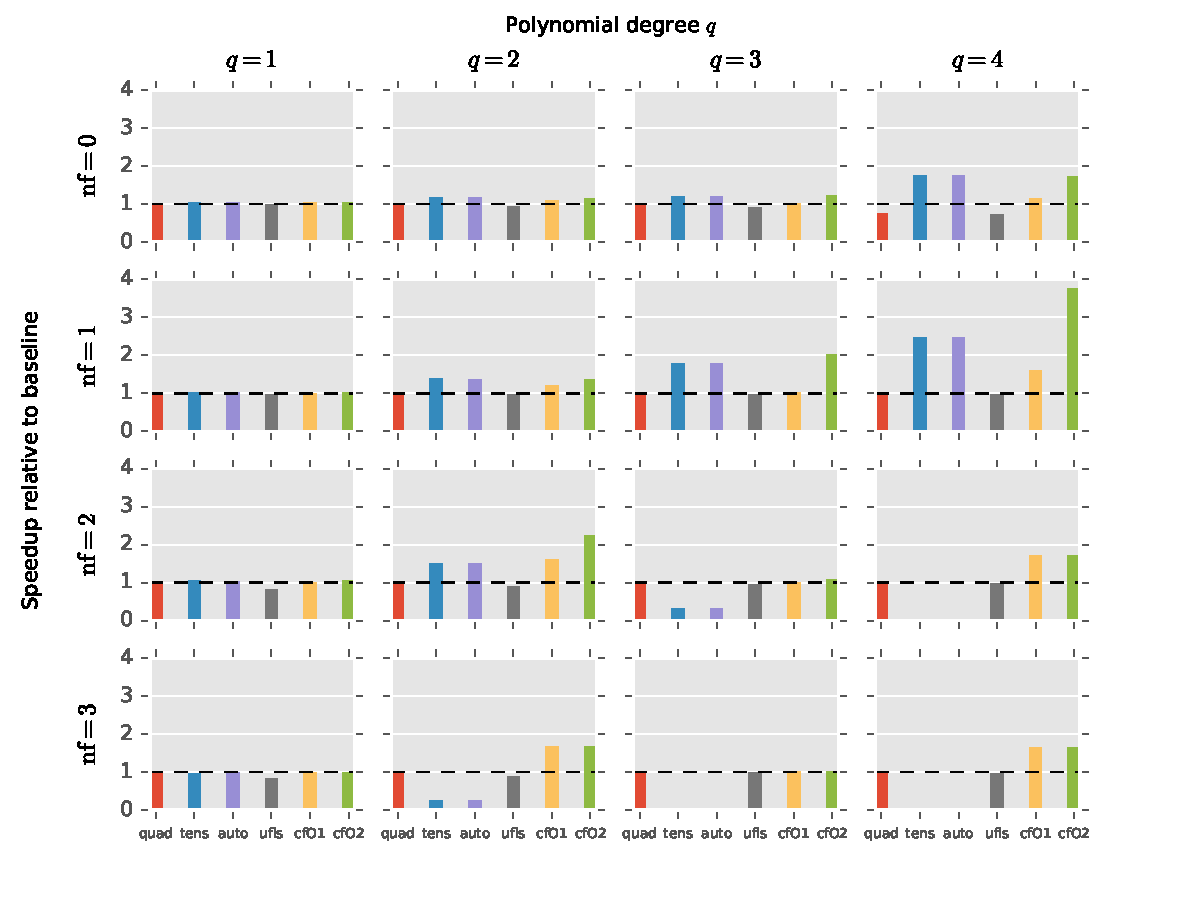
\includegraphics[scale=0.77]{perf-results/mass}}
\caption{Performance evaluation for the \textit{mass} matrix. The bars represent speed-up over the original (unoptimized) code produced by the FEniCS Form Compiler.}\label{fig:mass}
\end{figure}

\begin{figure}
 \makebox[\textwidth][c]{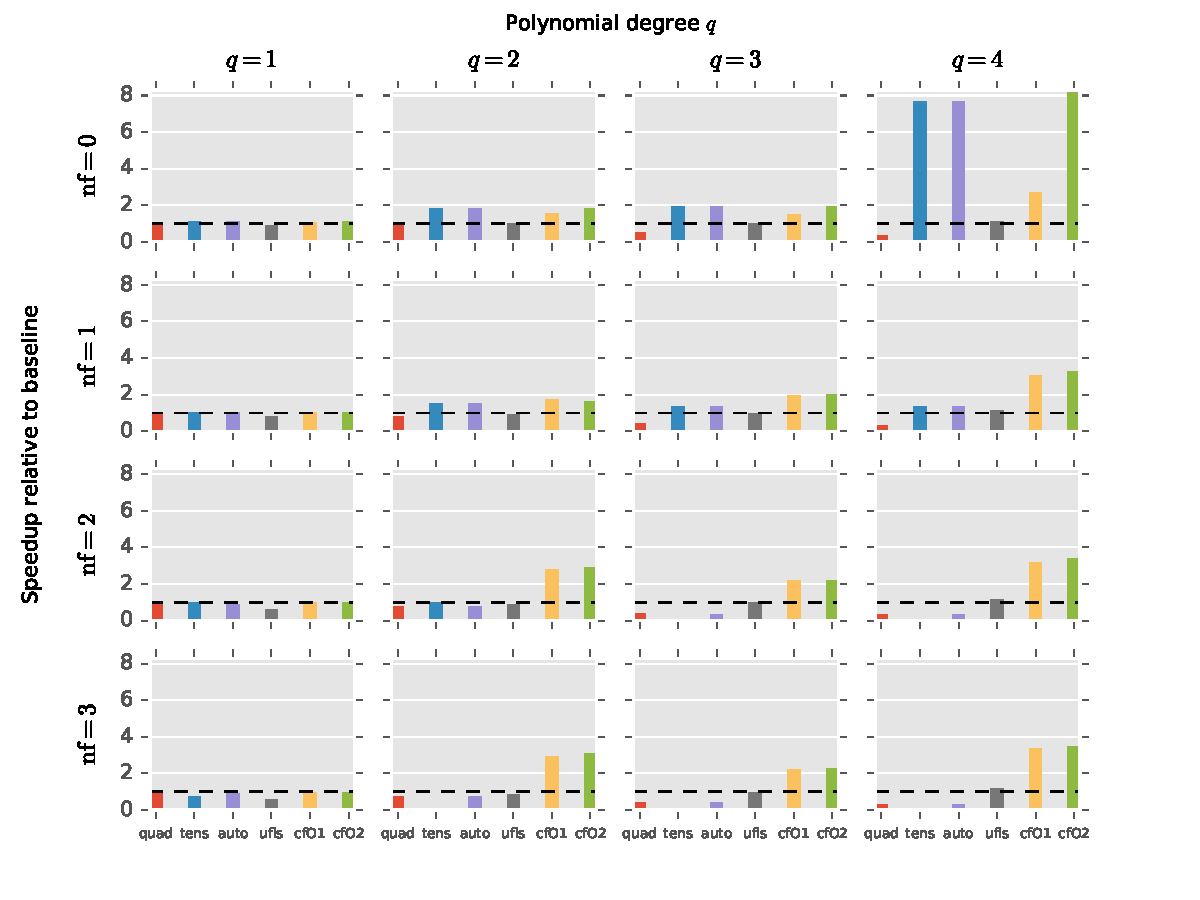
\includegraphics[scale=0.77]{perf-results/helmholtz}}
\caption{Performance evaluation for the bilinear form of a \textit{Helmholtz} equation. The bars represent speed-up over the original (unoptimized) code produced by the FEniCS Form Compiler.}\label{fig:helmholtz}
\end{figure}

\begin{figure}
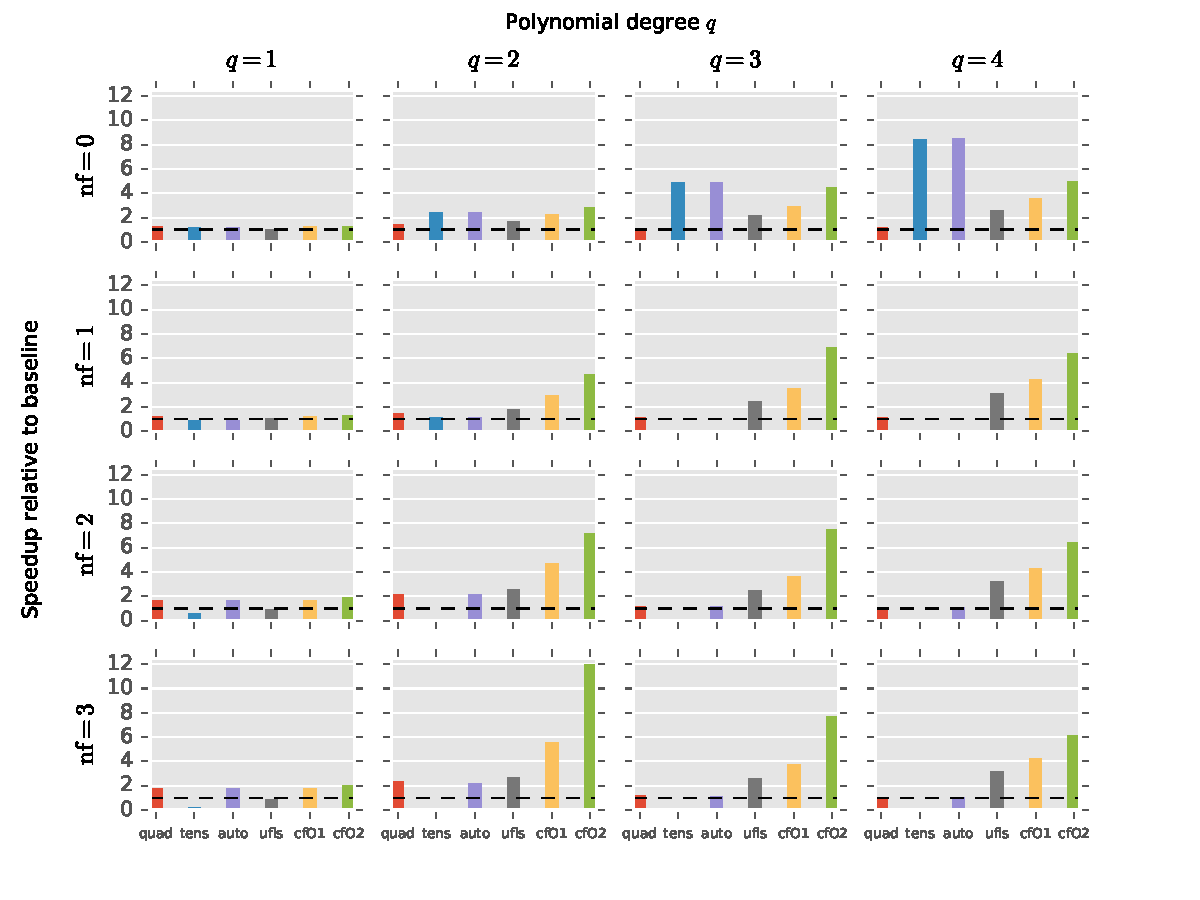
\includegraphics[scale=0.77]{perf-results/elasticity}
\caption{Performance evaluation for the bilinear form arising in an \textit{elastic} model. The bars represent speed-up over the original (unoptimized) code produced by the FEniCS Form Compiler.}\label{fig:elasticity}
\end{figure}

\begin{figure}
 \makebox[\textwidth][c]{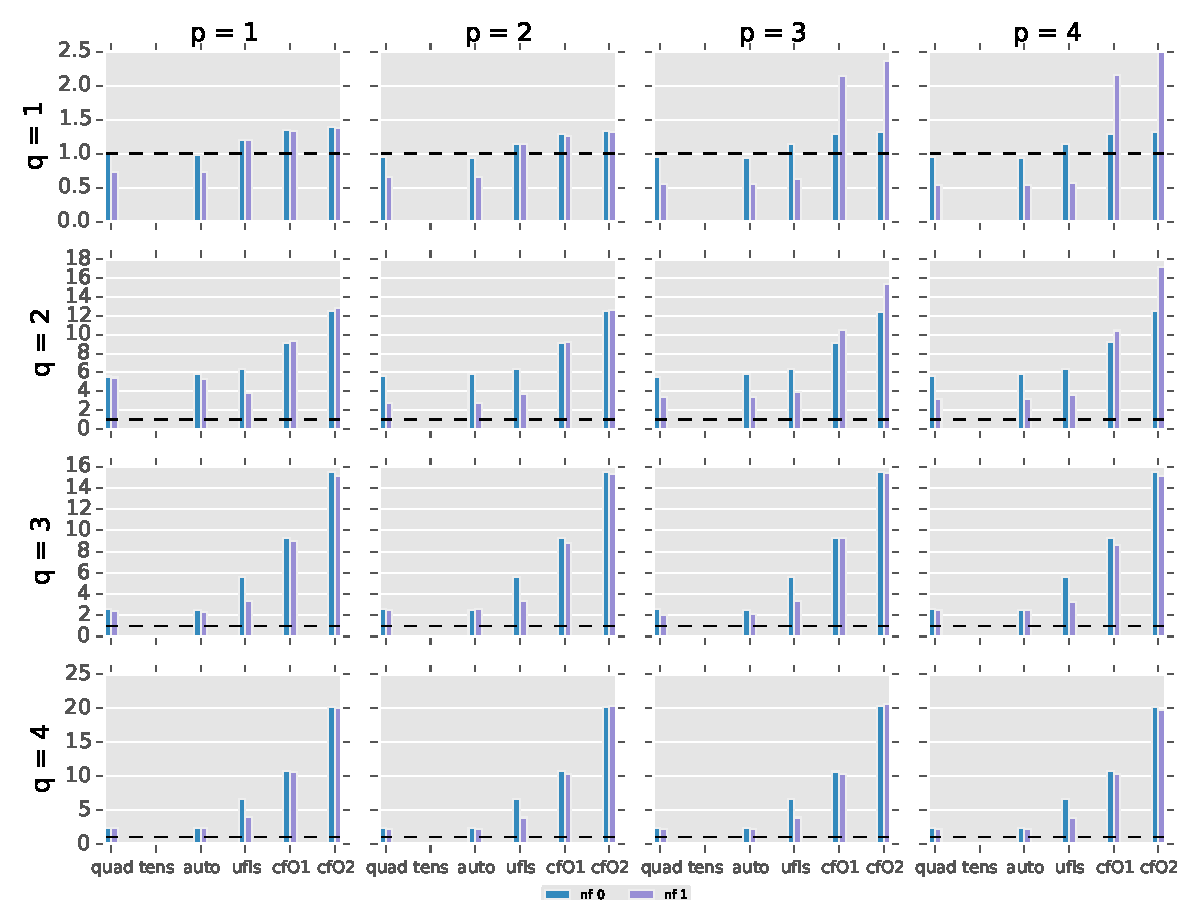
\includegraphics[scale=0.77]{perf-results/hyperelasticity}}
\caption{Performance evaluation for the bilinear form arising in a \textit{hyperelastic} model. The bars represent speed-up over the original (unoptimized) code produced by the FEniCS Form Compiler.}\label{fig:hyperelasticity}
\end{figure}

We report the results of our experiments in Figures~\ref{fig:mass},~\ref{fig:helmholtz},~\ref{fig:elasticity}, and~\ref{fig:hyperelasticity} as three-dimensional plots. The axes represent $q$, $nf$, and code transformation system. We show one subplot for each problem instance $\langle form, nf, q\rangle$, with the code transformation system varying within each subplot. The best variant for each problem instance is given by the tallest bar, which indicates the maximum speed-up over non-transformed code. We note that if a bar or a subplot are missing, then the form compiler failed at generating code because of either exceeding the system memory limit or unable to handle the form. 

The rest of the section is structured as follows: we provide insights about the main message of the experimentation; we comment on the impact of autovectorization; we explain in detail, individually for each form, the performance results obtained.

\paragraph{High level view}
The main observation is that our transformation strategy does not always guarantee minimum execution time. In particular, 5$\%$ of the test cases (3 out of 56, without counting marginal differences) show that \texttt{cfO2} was not optimal in terms of runtime. The most significant of such test cases is the elastic model with $[q=4, nf=0]$. There are two reasons for this. Firstly, low level optimization can have a significant impact on actual performance. For example, the aggressive loop unrolling in \texttt{tens} eliminates operations on zeros and reduces the working set size by not storing entire temporaries; on the other hand, preserving the loop structure can maximize the chances of autovectorization. Secondly, memory constraints are critical, particularly the transformation strategy adpopted when exceeding $T_H$. We will later thoroughly elaborate on all these aspects.

\paragraph{Autovectorization}
The discretizations employed result in inner loops and basis function tables of size multiple of the machine vector length. This, combined with the chosen compilation flags, promotes autovectorization in the majority of code variants. An exception is \texttt{quad} due to the presence of indirection arrays in the generated code. In \texttt{tens}, loop nests are fully unrolled, so the standard loop vectorization is not feasible; manual inspection of the compiled code suggests, however, that block vectorization (\cite{SLP-vect}) is often triggered. In \texttt{ufls}, \texttt{cfO1}, and \texttt{cfO2} the iteration spaces have similar structure (there are a few exceptions in \texttt{cfO2} due to zero-elimination), with loop vectorization being regularly applied, as far as we could evince from compiler reports and manual inspection of assembly code.

\paragraph{Mass}
We start with the simplest of the bilinear forms investigated, the mass matrix. Results are in Figure~\ref{fig:mass}. We first notice that the lack of improvements when $q=1$ is due to the fact that matrix insertion outweighs local assembly. As $q \geq 2$, \texttt{cfO2} generally shows the highest speed-ups. It is worth noting how \texttt{auto} does not always select the fastest implementation: \texttt{auto} always opts for \texttt{tens}, while as $nf \geq 2$ \texttt{quad} would tend to be preferable. On the other hand, \texttt{cfO2} always makes the optimal decision about whether applying pre-evaluation or not.  

\paragraph{Helmholtz}
As happened with the mass matrix problem, when $q=1$ matrix insertion still hides the cost of local assembly. For $q \geq 2$, the general trend is that \texttt{cfO2} outperforms the competitors. In particular, with
\begin{itemize}
\item $nf=0$, the adoption of pre-evaluation by \texttt{cfO2} results in increasingly notable speed-ups over \texttt{cfO1}, as $q$ increases; \texttt{tens} is comparable to \texttt{cfO2}, with \texttt{auto} making the right choice. 
\item $nf=1$, \texttt{auto} picks \texttt{tens}; the choice is however sub-optimal when $q=3$ and $q=4$. This can indirectly be inferred from the large gap between \texttt{cfO1/cfO2} and \texttt{tens/auto}: \texttt{cfO2} applies sharing elimination, but it avoids pre-evaluation. 
\item $nf=2$ and $nf=3$, \texttt{auto} reverts to \texttt{quad}, which would theoretically be the right choice (the flop count is much lower than in \texttt{tens} or what would be produced by pre-evaluation); however, the generated code suffers from the presence of indirection arrays, which break autovectorization and ``traditional'' code motion.
\end{itemize}

The sporadic slow-downs or only marginal improvements exhibited by \texttt{ufls} are imputable to the presence of sharing.

An interesting experiment we performed was relaxing the memory threshold by setting it to $T_H = L3_{size}$. We found that this makes \texttt{cfO2} generally slower as $nf \geq 2$, with a maximum slow-down of 2.16$\times$ with $\langle nf=2, q=2\rangle$. The effects of not having a sensible threshold could even be worse in parallel runs, since the L3 cache is shared by the cores.

\paragraph{Elasticity}
The results for the elastic model are displayed in Figure~\ref{fig:elasticity}. The main observation is that \texttt{cfO2} never triggers pre-evaluation, although in some occasions it should. To clarify this, consider the test case $\langle nf=0, q=2 \rangle$, in which \texttt{tens/auto} show a considerable speed-up over \texttt{cfO2}. \texttt{cfO2} finds pre-evaluation profitable -- that is, actually capable of reducing the operation count -- although it does not apply it because otherwise $T_H$ would be exceeded. However, running the same experiments with $T_H = L3_{size}$ resulted in a dramatic improvement, even higher than that of \texttt{tens}. Our explanation is that despite exceeding $T_H$ by roughly 40$\%$, the save in operation count is so large (5$\times$ in this problem) that pre-evaluation would anyway be the optimal choice. This suggests that our model could be refined to handle the cases in which there is a significant gap between potential cache misses and save in flops.

We also note that:
\begin{itemize}
\item the differences between \texttt{cfO2} and \texttt{cfO1} are due to systematic sharing elimination and the use of symbolic execution to avoid iteration over the zero-valued regions in the basis function tables
\item when $nf=1$, \texttt{auto} prefers \texttt{tens} to \texttt{quad}, which leads to sub-optimal operation counts and execution times
\item \texttt{ufls} generally shows better runtime behaviour than \texttt{quad} and \texttt{tens}. This is due to multiple facts, including avoidance of indirection arrays, preservation of loop structure, a more effective code motion.
\end{itemize}

\paragraph{Hyperelasticity}
In the experiments on the hyperelastic model, shown in Figure~\ref{fig:hyperelasticity}, \texttt{cfO2} exhibits the largest gains out of all problem instances considered in this paper. This is a positive aspect: it means that our transformation algorithm scales with form complexity. The fact that all code transformation systems (apart from \texttt{tens}) show quite significant speed-ups suggests several points. Firstly, the baseline is highly inefficient: with forms as complex as in this hyperelastic model, a trivial translation of integration routines into code should always be avoided since even one of the best general-purpose compilers available (Intel's on an Intel platform at maximum optimization level) is not capable of exploiting the structure inherent in the mathematical expressions generated. Secondly, the code motion strategy really makes a considerable impact. The sharing elimination performed by \texttt{cfO2} in each level of the loop nest ensures a critical reduction in operation count, which results is better execution times. In particular, at higher order, the main difference between \texttt{ufls} and \texttt{cfO2} is due to the application of this transformation to the multilinear loop nest. Clearly, the operation count increases with $q$, and so do the speed-ups. 



\section{Conclusions}
\label{sec:conclusions}
With this research we have set the foundation of optimal finite element integration. We have developed theory and implemented an automated system capable of applying it. The automated system, COFFEE, is integrated in Firedrake, a real-world framework for writing finite element methods. We believe the results are extremely positive. An open problem is understanding how to optimally handle non-linear loop nests. A second open problem is extending our methodology to classes of loops arising in spectral methods; here, the interaction with low level optimization will probably become stronger due to the typically larger working sets deriving from the use of high order function spaces. Lastly, we recall our work is publicly available and is already in use in the latest version of the Firedrake framework.

% Bibliography
\bibliographystyle{ACM-Reference-Format-Journals}
\bibliography{biblio}


\medskip

\end{document}
